\documentclass[12pt,a4paper]{report}

% --- Paquetes de Idioma y Codificación ---
\usepackage[utf8]{inputenc}
\usepackage[T1]{fontenc}
\usepackage[spanish, es-tabla]{babel}

% --- Diseño de Página ---
\usepackage{geometry}
\geometry{top=2.5cm, bottom=2.5cm, left=3cm, right=3cm}

% --- Matemáticas y Símbolos ---
\usepackage{amsmath, amssymb, amsthm}

% --- Colores y Cajas ---
\usepackage[dvipsnames]{xcolor}
\usepackage[most]{tcolorbox}

% Caption

\usepackage{caption}

% Gráficos

\usepackage{graphicx}

% Espaciadora

\newcommand{\esp}{\vspace{0.5cm}}

% promedio

\newcommand{\prom}[1]{\left\langle #1 \right\rangle}

% ket

\newcommand{\ket}[1]{| #1 \rangle}

% bra

\newcommand{\bra}[1]{\langle #1 |}

% braket

\newcommand{\braket}[2]{\langle #1 | #2 \rangle}

% Bibliografía

\usepackage[style=apa, backend=biber]{biblatex} % Estilo APA
\addbibresource{biblio.bib} % Nombre de tu archivo .bib

% Configuración de cajas personalizadas
\newtcolorbox{importante}{
	colback=red!5!white,
	colframe=red!75!black,
	title=Importante,
	fonttitle=\bfseries
}

\newtcolorbox{nota}{
	colback=blue!5!white,
	colframe=blue!75!black,
	title=Nota,
	fonttitle=\bfseries
}

% Definición de la caja de bibliografía
\newtcolorbox{bibliografia}{
	colback=gray!5!white,
	colframe=gray!75!black,
	title=Bibliografías útiles,
	fonttitle=\bfseries,
	breakable
}

% Socrative para óptica 2

\newtcolorbox{Socrative}{
	colback=orange!5!white,
	colframe=orange!75!black,
	title=Socrative,
	fonttitle=\bfseries,
	breakable
}

% Float

\usepackage{float}

% --- Hipervínculos ---
\usepackage{hyperref}
\hypersetup{
	colorlinks=true,
	linkcolor=blue,
	filecolor=magenta,      
	urlcolor=cyan,
}

% --- Datos del Documento ---
\title{Statistical Physics}
\author{Chengyu Jin}
\date{\today}

\begin{document}
	
	\maketitle
	
	\tableofcontents
	\newpage
	
	\chapter{Microscopic description}
	
	Statistical physics serves as the bridge that connects the microscopic world of atoms and molecules to the macroscopic phenomena observed in our everyday lives. At its core, this field is concerned with unraveling the mysteries of nature by understanding how countless microscopic particles, when aggregated, give rise to
	the familiar and predictable behaviour of macroscopic systems. This chapter provides us with the tools and knowledge necessary to comprehend the underlying dynamics of particles at the smallest scales. Here, we shift our focus from macroscopic observables like pressure and temperature to study individual particles – their motions, interactions, and the probabilistic nature of their behaviour. As we walk through the microscopic world, we will uncover the principles governing the behaviour of molecules and atoms. We will decipher the significance of concepts such as phase space, Hamiltonian mechanics, and quantum states, all of which play crucial roles in painting a vivid portrait of the microscopic universe. By the end of this chapter, you will possess a profound understanding of how microscopic details pave the way for macroscopic phenomena.
	
	\section{Classical Description}
	
	\begin{figure}[H]
		\centering
		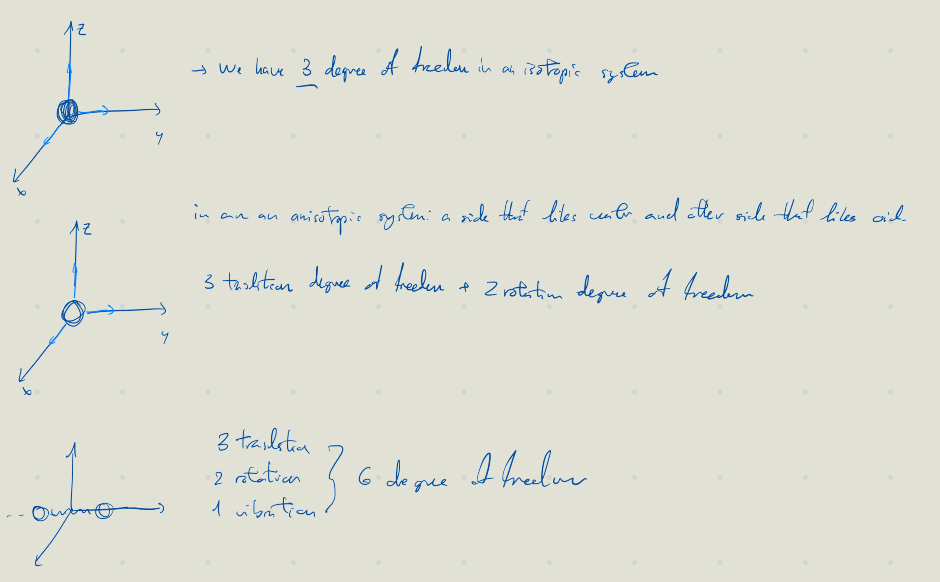
\includegraphics[width=0.7\textwidth]{IMG/degreeoffree.png}
	\end{figure}
	
	\esp
	
	
	\begin{enumerate}
		\item An isotropic atom has no rotational degrees of freedom , but only three translational degrees of freedom. Since any rotation of a perfectly symmetrical sphere constitutes an identity transformation, the orientation does not alter the particle's interaction potential. Consequently, the system’s energy remains invariant under rotation, meaning no thermal energy can be coupled to this motion, and the rotational degrees of freedom are effectively non-existent in the statistical count.
		\item An anisotropic atom of two side, one likes water and one likes oil has 2 rotational degrees of freedom and the three translational degrees of freedom. In this scenario, where the northern and southern hemispheres exhibit distinct interaction potentials, the perfect spherical symmetry is broken and replaced by axial symmetry. A rotation around the Z-axis (the axis of symmetry) leaves the configuration invariant, meaning it does not change the physical state. However, rotations around the X and Y axes alter the orientation of the hemispheres relative to their surroundings, creating distinguishable states. Consequently, we account for exactly two rotational degrees of freedom.
		\item A diatomic molecule has 3 translational,
		2 rotational and 1 vibrational (due to the distance between both particles) degrees of freedom.
	\end{enumerate}
	
	\esp
	
	\noindent \textbf{Just for curiosity}
	
	\esp
	
	\begin{tabular}{|c|c|c|c|}
		\hline
		Degrees of Freedom (s) & A (Atom $\implies$ N=1) & Linear Molecule & Non-linear Molecule \\
		\hline
		Traslational & 3(N) & 3 & 3 \\
		\hline
		Rotation & 0 & 2 & 3 \\
		\hline
		Vibration & 0 & 3N-5 & 3N-6 \\
		\hline
		Total & 3(N) & 3N & 3N \\
		\hline
	\end{tabular}
	
	\esp
	
	\noindent \textbf{The degree of freedom is always 3N}.
	
	\esp
	
	\begin{nota}
		In this chapter we will only treat particles as \textbf{simple spheres}.
	\end{nota}
	
	\esp

	
	\begin{figure}[H]
		\centering
		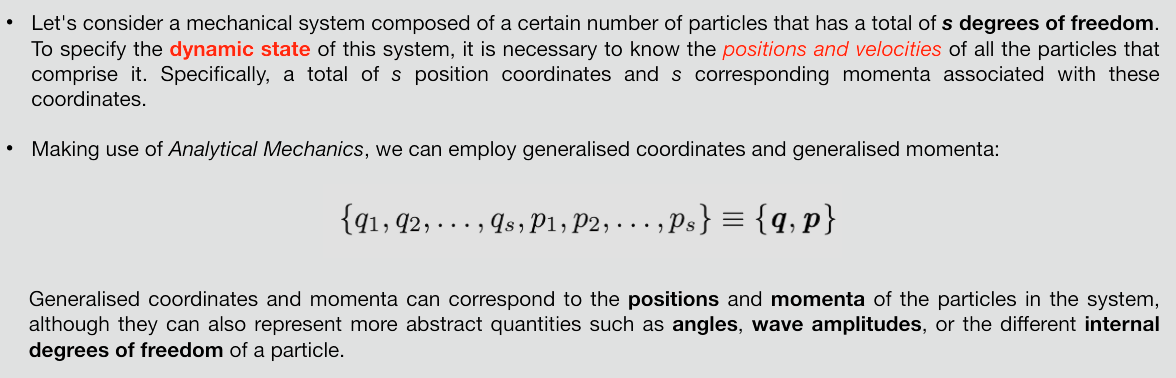
\includegraphics[width=0.7\textwidth]{IMG/classicdynamic.png}
	\end{figure}
	
	\esp
	
	In classical physics, the description of a system often involves a fundamental and powerful concept known as phase space, here indicated as $\Gamma$. Phase space provides a comprehensive mathematical framework for understanding and predicting the behaviour of physical systems. It is particularly essential in classical mechanics for analysing systems with complex configurations and interactions. Phase space provides physicists and engineers with a powerful tool for modelling and analysing complex systems. It allows us to visualise
	and study the system’s evolution over time by tracing its path through the multidimensional space. This approach simplifies the prediction of a system’s future behaviour, making it a fundamental concept in classical mechanics and other branches of physics. Understanding phase space is essential for tackling a wide range of problems, from the motion of celestial bodies to the behaviour of particles in a gas. It forms the basis for classical mechanics and serves as a foundation for more advanced topics in physics. At its core, phase space is a multidimensional mathematical space that offers a complete representation of the state of a physical system. Each point within phase space corresponds to a \textbf{unique state of the system}. The number of dimensions in phase space equals the number of \textbf{generalised coordinates} and \textbf{generalised momenta} required to define the system’s configuration. For example, in a system with s degrees of freedom, the corresponding
	phase space would be a 2s-dimensional space. This concept allows us to track the system’s evolution through all possible states by examining its trajectory in phase space.
	
	\esp
	
	\begin{figure}[H]
		\centering
		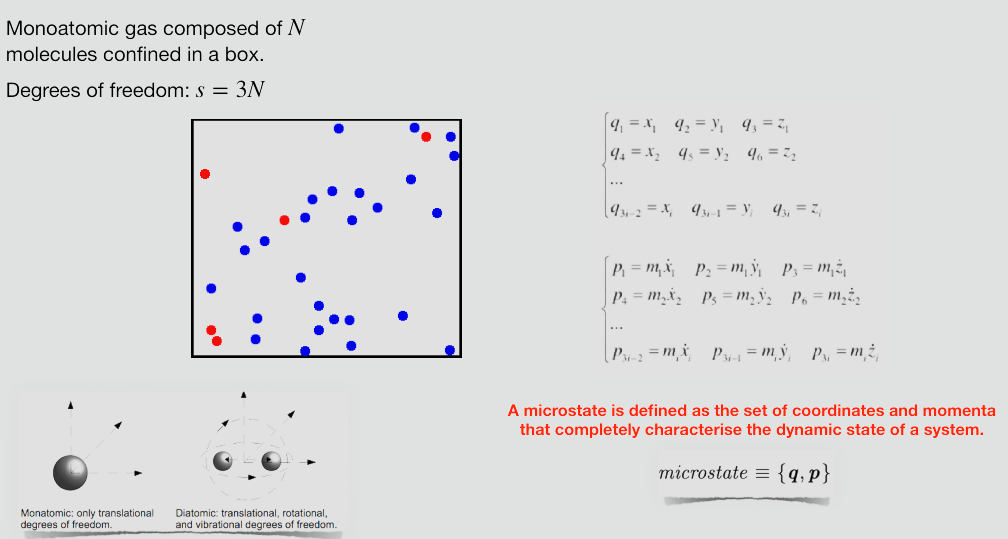
\includegraphics[width=0.7\textwidth]{IMG/examplemicrostate.png}
	\end{figure}

	\esp 
	
	Consider a monoatomic gas composed of N molecules confined within a box. In this case, the degrees of freedom are given by s = 3N. Its generalized coordinates for positions and momenta can be written as
	follows:
	
	\esp
	
	\noindent \textbf{Generalised coordinates}
	
	\esp
	
	$$
	\left\{
	\begin{aligned}
		q_1 &= x_1 & q_2 &= y_1 & q_3 &= z_1 \\
		q_4 &= x_2 & q_5 &= y_2 & q_6 &= z_2 \\
		\dots \\
		q_{3i-2} &= x_i & q_{3i-1} &= y_i & q_{3i} &= z_i
	\end{aligned}
	\right.
	$$

	\esp
	
	\noindent \textbf{Generalised momenta}
	
	\esp

	$$
	\left\{
	\begin{aligned}
		p_1 &= m_1 \dot{x}_1 & p_2 &= m_1 \dot{y}_1 & p_3 &= m_1 \dot{z}_1 \\
		p_4 &= m_2 \dot{x}_2 & p_5 &= m_2 \dot{y}_2 & p_6 &= m_2 \dot{z}_2 \\
		\dots \\
		p_{3i-2} &= m_i \dot{x}_i & p_{3i-1} &= m_i \dot{y}_i & p_{3i} &= m_i \dot{z}_i
	\end{aligned}
	\right.
	$$
	
	\esp
	
	In this representation, $q_i$ denotes the position coordinates, while $p_i$ corresponds to the momenta of the i-th particle within the system. These variables, combined with time, allow us to describe the complete state of the system dynamically.

	\esp 
	
	\noindent \textbf{Microstate Definition}
	
	\esp
	
	A microstate is defined as the set of coordinates and momenta that completely characterise the dynamic state of a system.
	
	\begin{equation}
		microstate \equiv \left\{\mathbf{q}, \mathbf{p}\right\} \equiv \left\{ q_1, q_2, \dots, p_1, p_2, \dots, p_s \right\}
	\end{equation}
	
	\subsection{Phase Space}
	
	\begin{figure}[H]
		\centering
		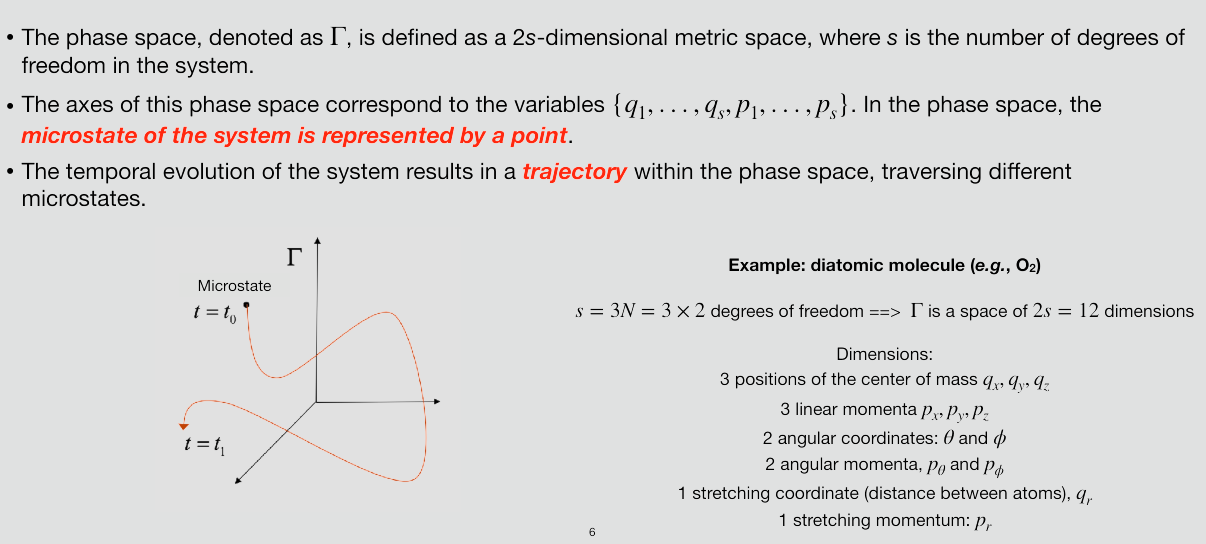
\includegraphics[width=0.7\textwidth]{IMG/phasespace.png}
	\end{figure}
	
	\esp
	
	The space of phases (or phase space), denoted as $\Gamma$, is defined as a 2s-dimensional metric space, where s is the number of degrees of freedom in the system. The axes of this phase space correspond to the variables $\left\{q_1, \dots , q_s, p_1, \dots , p_s\right\}$. In the phase space, the \textbf{microstate of the system is represented by a point}. Furthermore, the temporal evolution of the system results in a trajectory within the phase space, traversing different microstates.
	
	\esp
	
	\noindent \textbf{Example}. Representation of an oscillation in the phase space.
	
	\begin{equation*}
		F = -kx \implies m\ddot{x}=-kx \implies \ddot{x} + \frac{k}{m}x = 0
	\end{equation*}
	
	\esp
	
	\noindent Calling $\omega^2 = k/m$ we get the following $x(t)$ and $p(t)=m\dot{x}(t)$
	
	\esp
	
	\begin{eqnarray*}
		x(t) = C_1 \cos(\omega t) + C_2 \sin(\omega t)\\
		p(t) = - m\omega C_1 \sin(\omega t) + m\omega C_2 \cos(\omega t)
	\end{eqnarray*}
	
	\esp
	
	Using initial conditions, $x(t=0)=x_0$ and $p(t=0)=p_0$, we obtain the values of $C_1$ and $C_2$ which are $C_1=x_0$ and $C_2 = p_0/m\omega$. Replacing these values in our functions we get.
	
	\begin{eqnarray*}
		x(t) = x_0 \cos(\omega t) + p_0/m\omega \sin(\omega t)\\
		p(t) = - m\omega x_0 \sin(\omega t) + p_0 \cos(\omega t)
	\end{eqnarray*}
	
	\esp
	
	\noindent Multiplying $x(t)$ by $m\omega$, then square $x(t)$ and $p(t)$ and sums them we have
	
	\esp
	
	\begin{equation}
		m^2\omega^2x^2(t)+p^2(t)=m^2\omega^2x^2_0+p^2_0= cte
	\end{equation}
	
	\esp
	
	\noindent Let's analyse the units of the previous equation and let's repeat it after multiply both sides of the equation by $1/2m$.
	
	\esp
	
	\noindent $[m^2\omega^2x^2(t)]$ = $[kg\cdot m/s]^2$, \hspace*{0.3cm} $[p^2(t)]$ = $[kg\cdot m/s]^2$
	
	\esp
	
	\begin{equation}
		\frac{1}{2}m\omega^2x^2(t)+\frac{1}{2m}p^2(t)=\frac{1}{2}m\omega^2x^2_0+\frac{1}{2m}p^2_0= cte
		\label{eq:energyeq}
	\end{equation}
	
	\esp
	
	\noindent $[(m/2)\omega^2x^2(t)]$ = $[kg\cdot m^2/s^2]$ = [$N\cdot m$] = [$J$] , \hspace*{0.3cm} $[(1/2m)p^2(t)]$ = [$N\cdot m$]
	
	\esp
	
	\noindent We can notice that we obtain units of \textbf{energy}.
	
	\esp
	
	In the phase space, the oscillation motion has a graphic of an ellipse with semiaxis $\sqrt{2mC'}$ and $\sqrt{2C'/m\omega^2}$ with $C'$ the right side of the eq (\ref{eq:energyeq})
	
	\subsection{Dynamic functions}
	
	\begin{figure}[H]
		\centering
		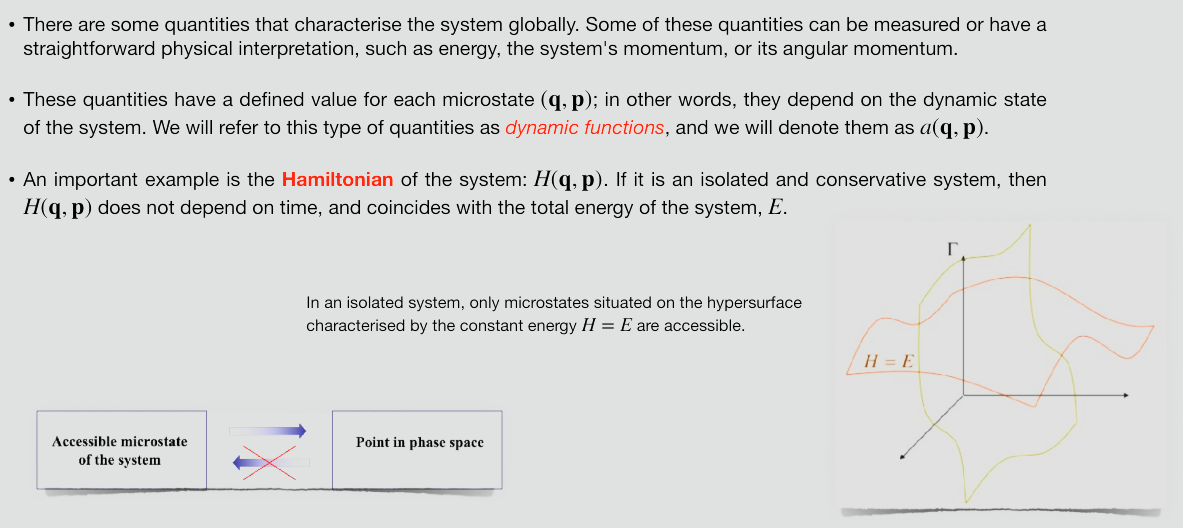
\includegraphics[width=0.7\textwidth]{IMG/dynamic.png}
	\end{figure}
	
	\esp
	
	In the field of statistical physics, numerous global properties are used to describe a system. Some of these properties are either directly measurable or possess straightforward physical interpretations. For instance, properties like energy, momentum, or angular momentum fall into this category. These properties assume specific values for each microstate $(\mathbf{q}, \mathbf{p})$, \textbf{indicating their dependence on the system’s dynamic state}. These types of properties are known as dynamic functions, typically denoted as $a(\mathbf{q}, \mathbf{p})$.
	
	\esp
	
	One significant example is the Hamiltonian of the system, often represented as $H(\mathbf{q}, \mathbf{p}))$. In the case
	of an isolated and conservative system, $H(\mathbf{q}, \mathbf{p})$ remains independent of time and corresponds to the total energy of the system, denoted as E:
	
	\begin{equation}
		H(\mathbf{q}, \mathbf{p}) = E
	\end{equation}
	
	\esp
	
	In an \textbf{isolated} system, only microstates situated on the hypersurface characterised by the constant energy
	$H = E$ are accessible. In a classical mechanical system, which is both isolated and conservative, the
	Hamiltonian function $H(\mathbf{q}, \mathbf{p})$ represents a crucial dynamic quantity. In this context, $H(\mathbf{q}, \mathbf{p})$ signifies the total energy of the system and remains independent of time. It encapsulates the intricate interplay of positions ($\mathbf{q}$) and momenta ($\mathbf{p}$) of all particles within the system.
	
	\subsection{Temporal Evolution of a Microstate}
	
	\begin{figure}[H]
		\centering
		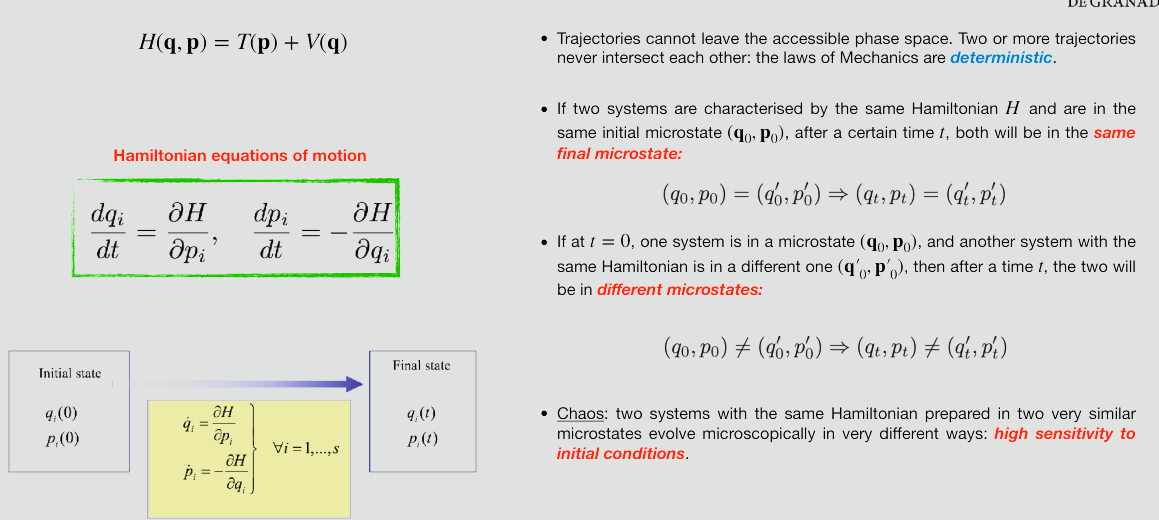
\includegraphics[width=0.7\textwidth]{IMG/tempevol.png}
	\end{figure}
	
	\begin{nota}
		Generally, the Hamiltonian can be decomposed as the contribution of kinetic energy and potential energy
		
		\begin{equation}
			H(\mathbf{q}, \mathbf{p}) = T(\mathbf{p}) + V(\mathbf{q})
		\end{equation}
	\end{nota}
	
	To understand the concept of the temporal evolution of a microstate within a dynamic system, we need to explore how the state of a system changes over time as it transitions between different microstates. Consider a classical mechanical system composed of a multitude of particles, each with its unique position and momentum. The complete description of the system at any given moment is provided by specifying the positions $q$ and momenta $p$ of all these particles. This set of 2s variables defines a microstate of the system at that particular instant. Now, let’s focus on how this microstate evolves over time. To do this, we need to
	introduce the concept of \textbf{equations of motion}. These equations, often derived from fundamental principles
	like Newton’s laws of motion, govern how the positions and momenta of particles change as a function of
	time. In classical mechanics, Hamilton’s equations of motion play a central role. These equations are a set
	of first-order differential equations that describe how the positions $q$ and momenta $p$ evolve over time:

	\esp
	
	\begin{equation}
		\frac{dq_i}{dt} =\frac{\partial H}{\partial p_i}, \quad \frac{dp_i}{dt} =-\frac{\partial H}{\partial q_i}
	\end{equation}

	\esp

	The solution to these equations of motion provides the trajectory of a microstate in the phase space $\Gamma$,
	which was introduced above. This trajectory represents how the microstate’s positions and momenta change
	as time progresses. Understanding the temporal evolution of microstates is fundamental for predicting
	the macroscopic behaviour of a system. By considering the \textbf{ensemble} of all possible microstates and their
	trajectories, statistical physics enables us to make probabilistic predictions about macroscopic observables,
	such as temperature, pressure, and entropy. These predictions are essential for understanding the behaviour
	of gases, liquids, solids, and many other complex systems in the realm of physics.
	
	\esp
	
	\begin{enumerate}
		\item Trajectories cannot leave the accessible phase space. Two or more trajectories never intersect each
		other: the laws of Mechanics are \textbf{deterministic}.
		\item If two systems are characterised by the same Hamiltonian H and are in the same initial microstate
		$(q_0, p_0)$, after a certain time $t$, both will be in the \textbf{same final microstate}.
		\begin{equation*}
			(q_0, p_0) = (q_0', p_0') \implies (q_t, p_t) = (q_t', p_t')
		\end{equation*}
		\item If at $t = 0$, one system is in a microstate $(q_0, p_0)$, and another system with the same Hamiltonian is in a different one $(q_0', p_0')$, then after a time $t$, the two will be in \textbf{different microstates}.
		\begin{equation*}
			(q_0, p_0) \neq (q_0', p_0') \implies (q_t, p_t) \neq (q_t', p_t')
		\end{equation*}
		\item Chaos: two systems with the same Hamiltonian prepared in two very similar microstates evolve mi-
		croscopically in very different ways: \textbf{high sensitivity to initial conditions}.
	\end{enumerate}

	\subsection{Temporal Evolution of a Dynamic Function}

	\begin{figure}[H]
		\centering
		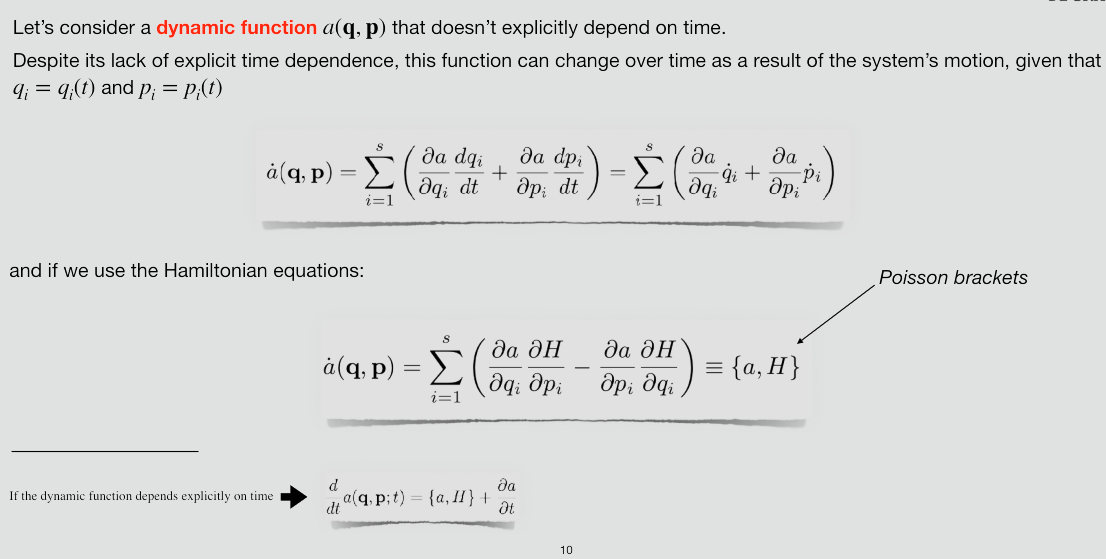
\includegraphics[width=0.7\textwidth]{IMG/dynaevol.png}
	\end{figure}

	\esp
	
	Let’s consider a \textbf{dynamic function} $a(\mathbf{q}, \mathbf{p})$ that doesn’t explicitly depend on time. Despite its lack of explicit time dependence, this function can change over time as a result of the system’s motion, given that $q_i = q_i(t)$ and $p_i = p_i(t)$.
	
	\esp
	
	\begin{equation}
		\dot{a}(\mathbf{q}, \mathbf{p}) = \sum_{i=1}^{s} \left( \frac{\partial a}{\partial q_i} \frac{dq_i}{dt} + \frac{\partial a}{\partial p_i} \frac{dp_i}{dt} \right) = \sum_{i=1}^{s} \left( \frac{\partial a}{\partial q_i} \dot{q}_i + \frac{\partial a}{\partial p_i} \dot{p}_i \right)
	\end{equation}

	\esp
	
	\noindent and if we use the Hamiltonian equations:
	
	\esp
	
	\begin{equation}
		\dot{a}(\mathbf{q}, \mathbf{p}) = \sum_{i=1}^{s} \left( \frac{\partial a}{\partial q_i} \frac{\partial H}{\partial p_i} - \frac{\partial a}{\partial p_i} \frac{\partial H}{\partial q_i} \right) \equiv \{a, H\}
	\end{equation}
	
	\esp
	
	where the brackets {} in the right-hand-side of the above equation are referred to as \textbf{Poisson brackets}. If the dynamic function depends explicitly on time, then

	\esp

	\begin{equation}
		\frac{d}{dt} a(\mathbf{q}, \mathbf{p}; t) = \{a, H\} + \frac{\partial a}{\partial t}
	\end{equation}
	
	\esp
	
	\begin{figure}[H]
		\centering
		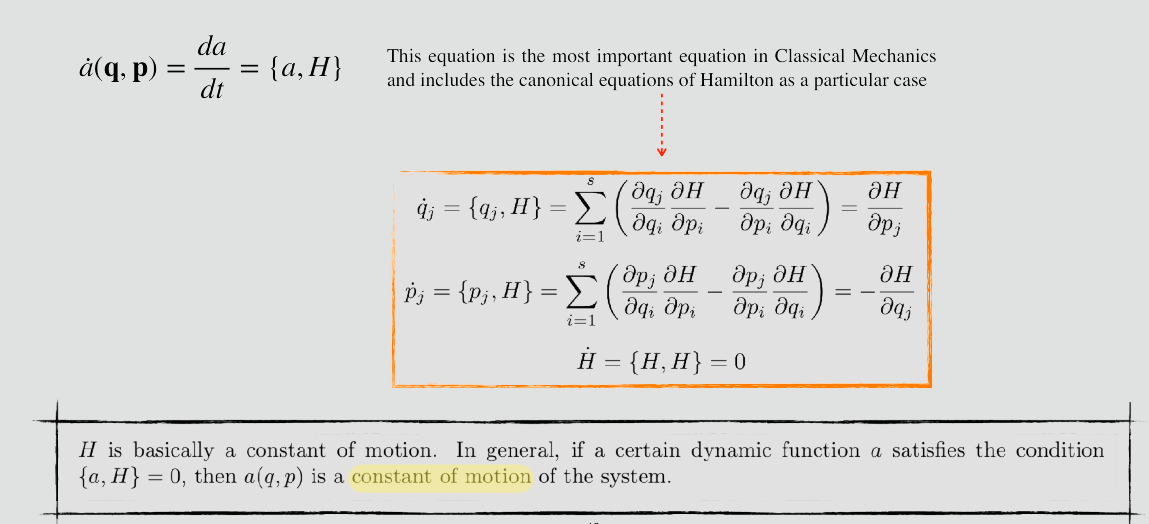
\includegraphics[width=0.7\textwidth]{IMG/dynaevol2.png}
	\end{figure}
	
	The above equation $\dot{a}(\mathbf{q}, \mathbf{p}) = {a, H}$ can be considered the most important equation in Classical Mechanics and includes the canonical equations of Hamilton as a particular case.
	
	\begin{equation}
		\dot{q}_j = \{q_j, H\} = \sum_{i=1}^{s} \left( \frac{\partial q_j}{\partial q_i} \frac{\partial H}{\partial p_i} - \frac{\partial q_j}{\partial p_i} \frac{\partial H}{\partial q_i} \right) = \frac{\partial H}{\partial p_j}
	\end{equation}
	
	\begin{equation}
		\dot{p}_j = \{p_j, H\} = \sum_{i=1}^{s} \left( \frac{\partial p_j}{\partial q_i} \frac{\partial H}{\partial p_i} - \frac{\partial p_j}{\partial p_i} \frac{\partial H}{\partial q_i} \right) = -\frac{\partial H}{\partial q_j}
	\end{equation}
	
	\begin{equation}
		\dot{H} = \left\{H, H\right\} = 0
	\end{equation}
	
	\esp
	
	H is basically a constant of motion. In general, if a certain dynamic function a satisfies the condition
	$\left\{a, H\right\} = 0$, then $a(\mathbf{q}, \mathbf{p})$ is a \textbf{constant of motion} of the system.
	
	\esp
	
	Some points of discussions:
	
	\begin{enumerate}
		\item  It is important to note that classical mechanics provides a well-defined and detailed microscopic description based on Newton’s laws. However, in general, we can only obtain a formal solution for the microscopic behaviour of the system due to:
		\begin{enumerate}
			\item The \textbf{impossibility of experimentally determining} the initial conditions of $\sim 10^{23}$ particles
			\item The \textbf{mathematical and numerical impossibility of solving} $\sim6\times10^{23}$ differential equations.
		\end{enumerate}
		\item An interesting question arises: Even if we could solve the equations, how is it possible for thermodynamics, for example, to emerge from such dynamic complexity? Would such a solution provide true
		understanding? Sometimes, knowing the analytical solution to a complex problem does not necessarily
		mean understanding what is happening.
		\item Microscopic Time Reversibility. The microscopic dynamic equations (Hamilton’s equations) are temporally reversible. This is demonstrated by reversing the sign of all momenta and the sign of time in the Hamiltonian equations, and observing that they remain invariant. How could this process generate
		irreversible macroscopic laws?
	\end{enumerate}
	
	\section{Quantum Description}
	
	\begin{figure}[H]
		\centering
		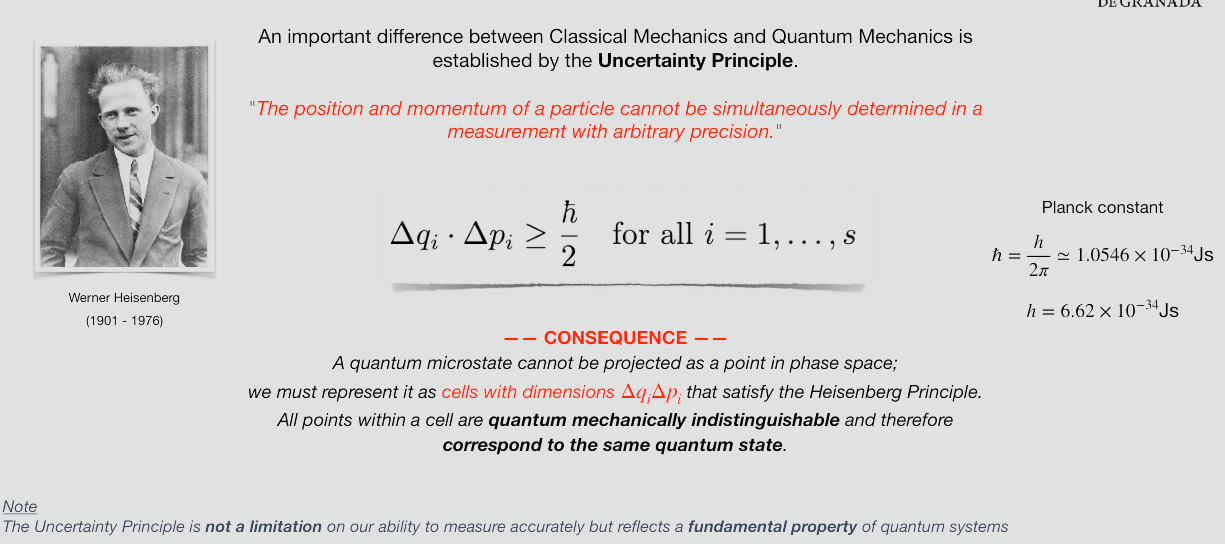
\includegraphics[width=0.7\textwidth]{IMG/uncertaintyp.png}
	\end{figure}

	One fundamental distinction between Classical Mechanics and Quantum Mechanics (QM) lies in the Uncertainty Principle, a concept introduced by Werner Heisenberg (1901 - 1976). This principle asserts that the precision with which we can simultaneously measure the position and momentum of a particle is \textbf{fundamentally limited}. In mathematical terms, it can be expressed as:
	
	\begin{equation}
		\Delta q_i \cdot \Delta p_i \geq \frac{\hbar}{2} \quad \text{for all}\ i=1,\dots,s
	\end{equation}
	
	\esp
	
	where $\Delta q_i$ represents the uncertainty in position, $\Delta p_i$ signifies the uncertainty in momentum, and $\hbar = h/2\pi = 1.054571817\dots × 10^{-34}$ J s (or, equivalently, J Hz$^{-1}$) denotes the reduced Planck constant, being $h$ the Planck constant. This principle has profound implications for our understanding of the behaviour of particles at the quantum level. It implies that we cannot precisely know both the position and momentum of a particle simultaneously, no matter how advanced our measurement tools become. In a semiclassical view, this would correspond to having ”fuzzy points” in phase space, with a volume proportional to $\hbar$.
	
	\esp 
	
	\noindent Let’s discuss some key features of this principle:

	\begin{enumerate}
		\item The Uncertainty Principle is a cornerstone of quantum theory and has led to a host of fascinating and counterintuitive phenomena, such as \textbf{wave-particle duality} and the \textbf{quantisation} of energy levels. It fundamentally challenges our classical intuition and underlines the inherent probabilistic nature of
		quantum systems.
		\item The principle implies that there is an \textbf{inherent limit} to how precisely both the position and momentum of a particle can be known simultaneously. In other words, the more accurately we know the position of a particle, the less accurately we can know its momentum, and vice versa.
		\item It fundamentally challenges classical physics, which assumes that it is possible to precisely determine both position and momentum. In QM, measurements are \textbf{inherently probabilistic}. Knowing the position of a particle precisely means that its momentum becomes highly uncertain, and vice versa.
		\item The Uncertainty Principle is intimately connected to the concept of \textbf{wave-particle duality}. It implies that particles, such as electrons and photons, exhibit both particle-like and wave-like behaviour. The more precisely you try to determine their position, the more you disturb their momentum, and vice.
		\item The Uncertainty Principle has wide-ranging implications in QM and plays a crucial role in the behaviour of subatomic particles. It has practical consequences in various quantum technologies, including quantum computing and quantum cryptography.
		versa.
		\item Beyond its mathematical and physical significance, the Uncertainty Principle has profound philosophical implications. It challenges our classical intuitions about the determinism of physical systems and raises questions about the nature of reality at the quantum level.
	\end{enumerate}
	
	\esp
	
	\begin{figure}[H]
		\centering
		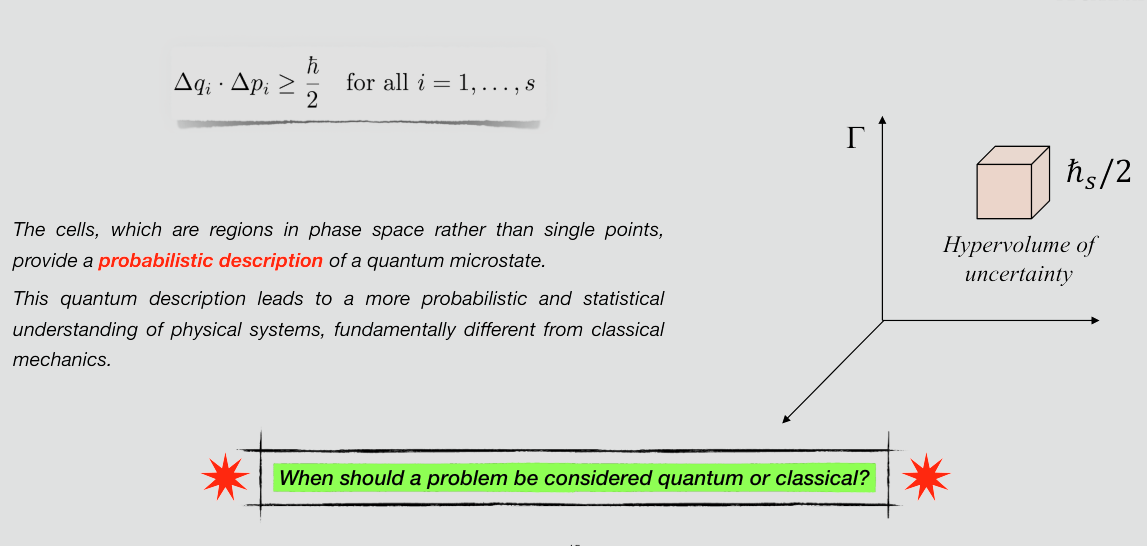
\includegraphics[width=0.7\textwidth]{IMG/uncertaintyp2.png}
	\end{figure}
	
	\esp
	
	In summary, the Uncertainty Principle is a foundational concept in QM, highlighting the fundamental
	limits on our ability to precisely know certain properties of particles. It underscores the probabilistic nature of quantum systems and has revolutionised our understanding of the behaviour of matter and energy at
	the smallest scales. An important consequence of the Uncertainty Principle is that a quantum microstate
	cannot be projected as a point in phase space. The classical description uses the concept of phase space,
	where each point represents a unique microstate of the system, specified by the generalised coordinates
	($q$) and momenta ($p$). Instead, we must depict a quantum microstate as cells with dimensions $\Delta q_i\Delta p_i$ that satisfy Heisenberg’s Uncertainty Principle. Consequently, within a cell in phase space, all points are quantum mechanically indistinguishable and correspond to the same quantum state. These \textbf{cells}, which are regions in phase space rather than single points, provide a probabilistic description of a quantum microstate. This quantum description leads to a more probabilistic and \textbf{statistical understanding of physical systems}, fundamentally different from classical mechanics. It is essential for understanding the behaviour of particles at the atomic and subatomic levels, where classical mechanics fails to provide an accurate description of their dynamics.

	\subsection{When should a problem be considered quantum or classical?}

	\begin{figure}[H]
		\centering
		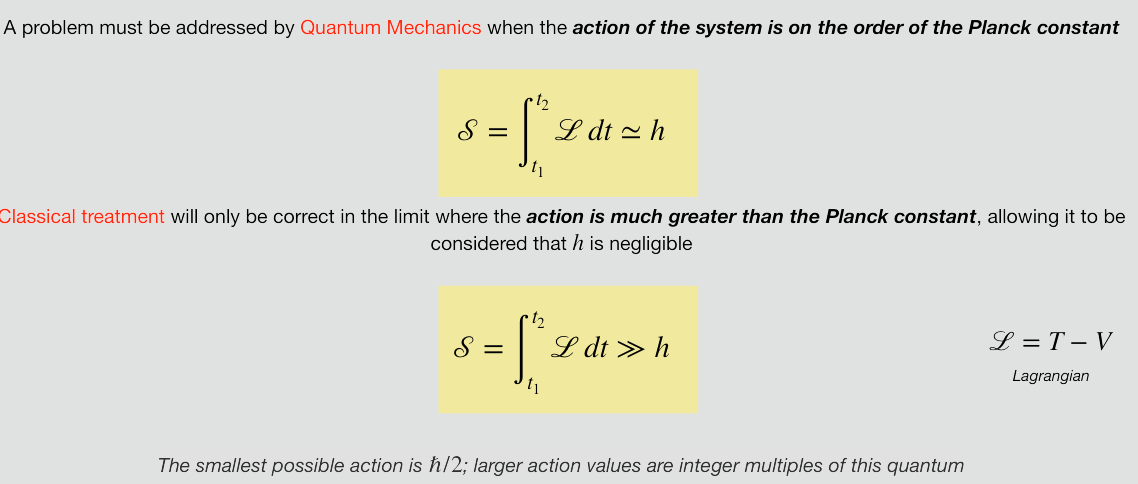
\includegraphics[width=0.7\textwidth]{IMG/qp.png}
	\end{figure}
	
	\esp
	
	The distinction between a problem that should be treated quantum mechanically or classically depends on the scale and characteristics of the system studied. QM is fundamental when dealing with microscopic systems, such as atoms, molecules, and subatomic particles. At these scales, quantum effects dominate, and classical mechanics becomes inadequate to describe their behaviour accurately. Classical mechanics, on the other hand, works well for macroscopic systems, where quantum effects are negligible and the classical approximation is valid. More quantitatively, a problem must inevitably be \textbf{addressed using QM} when the \textbf{action of the system is on the order of Planck’s constant}, $h = 6.62 \times 10^{-34}$ J s.
	
	\esp
	
	\begin{figure}[H]
		\centering
		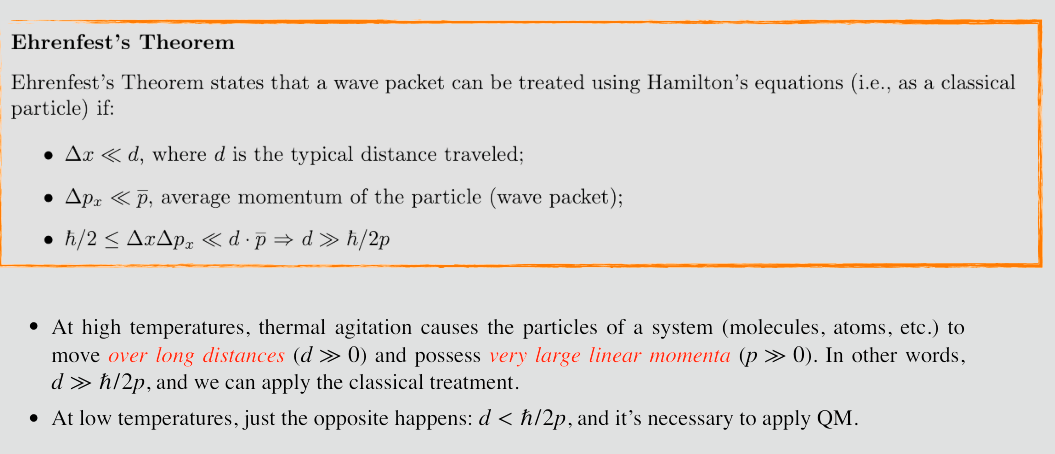
\includegraphics[width=0.7\textwidth]{IMG/ehren.png}
	\end{figure}
	
	\noindent \textbf{Ehrenfest’s Theorem}
	
	\esp
	
	Ehrenfest’s Theorem states that a wave packet can be treated using Hamilton’s equations (i.e., as a classical
	particle) if:
	
	\begin{enumerate}
		\item $\Delta x \ll d$, where $d$ is the typical distance traveled.
		\item $\Delta p_x \ll \bar{p}$, average momentum of the particle (wave packet)
		\item $\hbar/2\leq \Delta x\Delta p_x \ll \cdot \bar{p} \implies d \gg \hbar/2p$
	\end{enumerate}
	
	At high temperatures, thermal agitation causes the particles of a system (molecules, atoms, etc.) to move
	over long distances $(d \upuparrows)$ and possess very large linear momenta $(p \upuparrows)$. In other words, $d \gg \hbar/2p$, and we can apply the classical treatment. At low temperatures, just the opposite happens: $d < \hbar/2p$, and it’s necessary to apply QM. \textbf{When can we assume that temperature is high enough} to apply classical formalism? Thereis no single answer to this question; it \textbf{depends on the type of system}. For a gas of atoms/molecules, room temperature (300 K) is already high enough to consider the system as classical. For a gas of electrons in a metal at room temperature, the system still exhibits strong quantum behaviour. For most solids at room temperature, classical behaviour holds true; at low temperatures (below 100 K), quantum effects become
	relevant. For liquid Helium II (which is achieved at temperatures very close to absolute zero), a quantum
	treatment is necessary.
	
	\subsection{State Representation in QM}
	
	\begin{figure}[H]
		\centering
		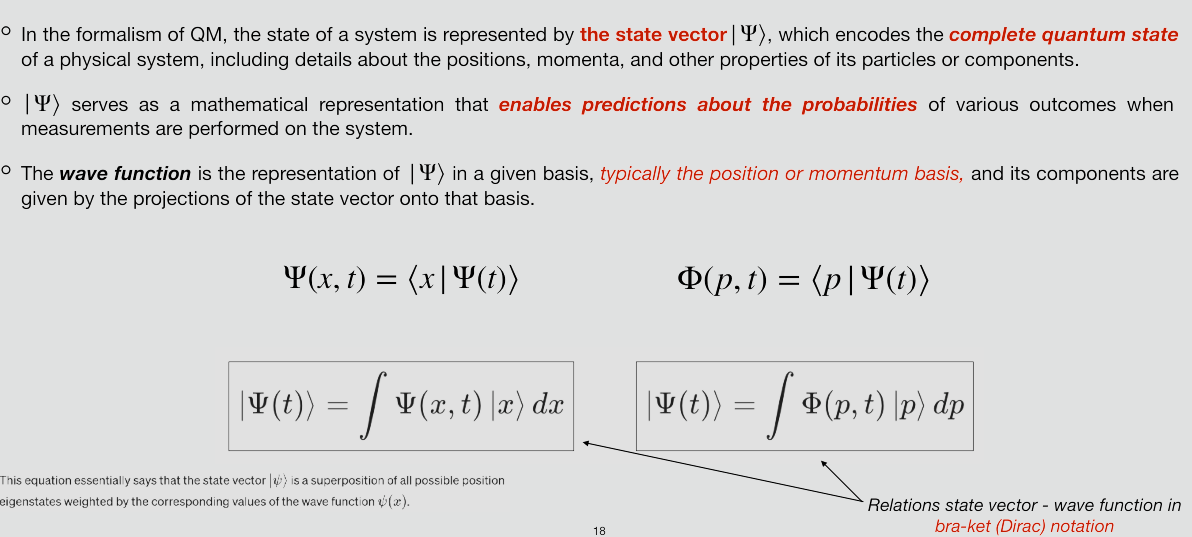
\includegraphics[width=0.7\textwidth]{IMG/staterep.png}
	\end{figure}
	
	In the formalism of QM, the state of a system is represented by a vector $\ket{\Psi}$ that encodes the \textbf{complete quantum state} of a physical system, including details about the positions, momenta, and other properties of its particles or components. It serves as a mathematical representation that \textbf{enables predictions about the probabilities} of various outcomes when measurements are performed on the system. At a particular instant of time, the components of this vector represent the values of the corresponding \textbf{wave function}
	
	\esp
	
	\begin{equation}
		\Psi = \Psi(q_1,\dots,q_s,t)
	\end{equation}
	
	\esp
	
	where $s$ is the number of degrees of freedom. The link between state vector and wave function, due to the extremely large number of represented values, is better expressed as an integral. In bra–ket (Dirac) notation,
	this vector is written as
	
	\esp
	
	\begin{equation}
		\ket{\Psi (t)} = \int \Psi(x,t)\ket{x} dx
	\end{equation}
	
	\esp
	
	By manipulating and evolving the wave function using quantum operators, one can make predictions about
	the behaviour of quantum systems, including particles like electrons, atoms, and molecules. The set of all
	states or wave functions possesses the structure of a \textbf{Hilbert space} $\hat{H}$, which is a complex vector space with an inner product that allows for the mathematical treatment of quantum states, operations, and measure-
	ments. This Hilbert space structure provides the mathematical framework for the description of quantum
	states and their evolution over time.
	
	\esp
	
	The main difference between phase space in classical mechanics and configuration space in QM lies in how they represent the state of a physical system and how variables are handled. Let’s look at this difference in more detail.
	
	\printbibliography[title={Bibliografía}]
\end{document}